\documentclass[11pt]{article}
\usepackage[english]{babel}
\usepackage{inputenc}
\usepackage{multicol}
\usepackage{flushend}
\usepackage{fullpage}
\usepackage{epsfig}
\usepackage{caption}
\captionsetup[table]{labelsep=period}
\usepackage{multirow}
\usepackage{mathtools}
\usepackage{xcolor}
\DeclarePairedDelimiter{\ceil}{\lceil}{\rceil}

\topmargin=-0.2in
\textheight=9.5in

\pagestyle{empty}

\begin{document}

\centerline{CSCE 614 (Fall 2020) \hfill Uwacu and Elsheimy}
\medskip
\centerline{\bf Computer Architecture}
\medskip

\centerline{\bf  Project report: }

\bigskip

\centerline{\bf Exploring Predictive Replacement Policies for Instruction Cache and Branch Target Buffer}

\bigskip

\centerline{\bf Diane Uwacu and Fatmaelzahraa Elsheimy}

\bigskip

\begin{abstract}
Many of the new-era processors support fetching instructions with instruction cache and branch target buffer. I-Cache and branch target buffer have limited capacities and
therefore, different types of replacement policies are being explored to reduce the misses in I-cache and BTB. In this project, we implement a new policy Global History Reuse 
Prediction (GHRP), a replacement policy that uses the history of previous instructions and behaviour predict and evict dead blocks. GHRP is implemented in the main paper using
Championship Branch Prediction simulator, but we try to implement it using Zsim to test the easiness of implementing the new policy in different simulators. GHRP’s performance
is compared against the famous policy LRU (Least recently used) and SRRIP(static re-reference interval prediction). Using Championship simulator, GHRP reduces the I-cache misses (MPKI) by 18% 
over LRU policy on a 662 industrial workloads. In Zsim, LRU data is collected over PARSEC benchmark and the results are speculated from the Championship results.
\end{abstract}

\section{Introduction} 
\label{sec:introduction}

Current processors need efficient instruction fetch for high performance. There are two main structures that the processor rely on for efficient fetching: I-cache and branch
target buffer. The instruction cache (I-cache) keeps record of recently used instructions, and the branch target buffer (BTB) caches targets of previously taken branches.
Therefore, the I-cache helps in improving instruction throughput and latency. Branch target buffer improves latency because of branch target-recomputation. This 
paper\cite{samira-ISCA18} explores efficient replacement policies at the I-cache and BTB levels. Samira et-al introduces a new idea for policy replacement called Graph History
Reuse Prediction. This algorithm is based on the history of past instruction addresses and behaviour in order to predict dead blocks in an efficient way. Predicting dead blocks
is very important as they free up space for other blocks that might be used in the future. A block is said to be dead if it is not going to be used before eviction. A block is 
said to be live if it is going to be used before eviction. Samira et-al have done a survey on the current implemented policies such as LRU, SSRIP..etc and tried to find a 
better policy. Most of the work on _cache optimization focused on instruction prefetching and block reordering. Many of these solutions didn’t lead to good  outcome as it 
resulted in large overhead or high MPKI. Similarly, most of the work on BTB optimization focused on the design structure or using different replacement policy. Again, the 
results weren’t that satisfactory. 
Samira et-al first, tried to apply PC-based predictor that uses set-sampling for Cache behavior generalization, however, when being applied on I-cache and BTB, they haven’t 
seen prominent results and hence, this idea was discarded. On the other side,  based on the survey done over all current replacement policies, they noted that that sequences of
recently accessed instructions correlate with the likelihood of block reuse. Their proposes policy results in a prominent improvement in cache efficiency and overall 
performance. They evaluated seven recent replacement policies and compared them based on average MPKI values. While, Samira et al applied their policy on Championship 
simulator. We have tried applying it on Zsim to test the ease of implementation of the policies in different simulators and compare the results using different benchmark; 
PARSEC.


\section{Background}
\label{sec:background}


\section{Work Description}
\label{sec:proposed}

\section{Evaluation}
\label{sec:timeline}

\subsection{Experimental Setup}

\subsection{Experimental Results and Discussion}
In order to compare the efficiency of the GHRP policy, it was implemented on two different simulators; Champ and Zsim. In the paper, Samira et al implement the policy using
Champ and comparing it with other policies such as LRU, and SRRIP on industrial benchmarks. In our project, we tried implementing on Zsim and comparing the results against 
SRRIP and LRU on PARSEC benchmark. Unfortunately, due to Zsim architecture and the way the policies are implemented. It was difficult to implement the GHRP policy in the 
current Zsim architecture. We collected data from Samira et al as well as collected data from the  LRU AND SRRIP on PARSEC and we speculated the results by GHRP. In figure 1,
It shows the results of the implementation of different policies on an 8-way 64KB I-cache with 64B blocks using Champ simulator. Figure 1 shows the results of these policies in
relative to the MPKI of the LRU. On average of the 662 workloads, GHRP has a lower MPKI average of 0.86 compared with 1.02 for SRRIP and 1.10 for SDBP. By percentage, GHRP 
improves the average MPKI by 18% over LRU and 12% over SRRIP. In the 2nd figure, Samira et al explored other configuration of the I-cache. In figure 2,  it shows various 
combinations of 8KB,  16KB, 32KB and 64KB caches with 64B blocks with 4-way or 8-way associativity. It can be clearly seen how GHRP outperformed all other policies. LRU has
performed the worst results by average of 10% less than other policies. GHRP has reduced the average of the MPKI by 14% compared to the LRU results.
Using Zsim, GHRP is compared against LRU and SRRIP on PARSEC benchmark. The MPKI value is calculated using the following equations:  
total misses = mGETS + mGETXIM + mGETXSM

MPKI = (total misses/total instruction)*1000
Where mGETS are misses of the GETS , mGETXIM are the
misses of GETXI => M, and mGETXSM are the misses
of the GETXS => M .

\begin{figure}[h]
	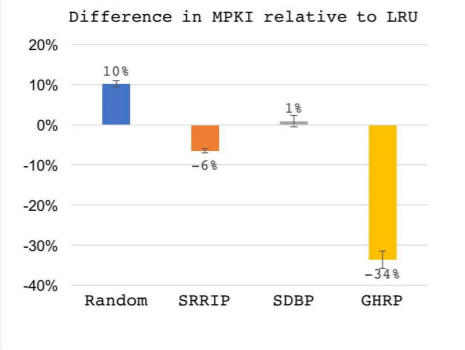
\includegraphics[width=1\textwidth]{report1.PNG}
	\includegraphics[width=1\textwidth]{reportresults.PNG}
\end{figure}

Figures 3 and 4 display the results of the policies over the PARSEC benchmarks. The value of the MPKI for each policy was calculated using the above mentioned equations and
recorded in figure 3. It can be clearly shown the LRU has done the worst compared to all of them. SRRIP has done better than LRU by average of 10%. According to Samira’s 
results, the GHRP is expected to outperform both LRU and SRRIP by average of 8% when compared with the previous results from figures 1 and 2. 
The analysis behind such results is due to the algorithm and the core idea of GHRP. GHRP targets the removal of dead blocks/BTB entries by using the history of past 
instructions addresses and behavior. LRU just uses information based on the last recently used block, which isn’t really efficient to detect dead blocks especially when it does
not think that the most recent entry will be re-referenced in
the near-immediate future. In results, LRU is inefficient especially with applications that its referenced mainly in the distant future. LRU replaces the blocks very 
frequently. 
 SSRIP uses lower hardware overhead and deals better with applications with larger working sets and applications with references in the distant future than LRU. SSRIP has two 
kinds of priorities: Hit priority and Frequency priority. For this project, the Hit priority one was implemented. Therefore, it can be deduced that many of the PARSEC 
benchmarks have blocks that are referenced in the distant future and that’s why SRRIP outperformed LRU. For GHRP, it can predict dead blocks in application with larger worker 
sets and references in the distant future better than both SRRIP and LRU. SRRIP uses 2 bits per cache block to store 2^2 prediction values (RRVP)for scan resistant, which means
a block has 4 chances before being evicted. GHRP doesn’t face this problem as it bases its prediction on indexing a table of counters with a signature generated by correlated 
it to data from previous history. The final prediction is passed by majority vote which further improves the assurance of the prediction. Hence, a block has a better chance to 
stay in cache before being evicted. Overall, GHRP better predict dead blocks than SRRIP and LRU. 

\begin{figure}[h]
	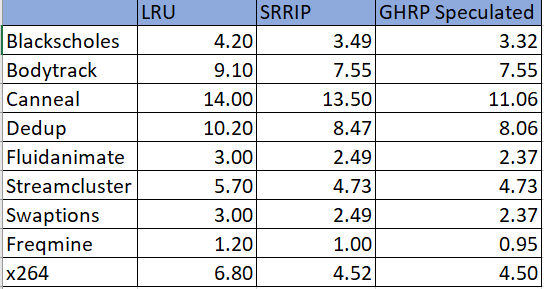
\includegraphics[width=1\textwidth]{MPKI1.PNG}
	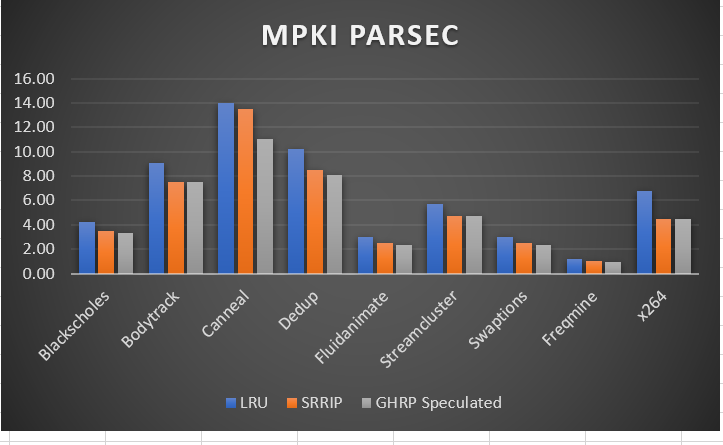
\includegraphics[width=1\textwidth]{MPKI2.PNG}
\end{figure}

\section{Conslusion and Future Work}

{%\scriptsize
	\bibliographystyle{abbrv}
	\bibliography{references}
	}

\end{document}



